\chapter{Umsetzung}
\label{ch:S5_Umsetzung}

\section{Erläuterung des Softwaretechnischen Entwurfs}
\label{ch5:s:Entwurf}

Für die Softwaretechnische Umsetzung wurden zunächst die Anforderungen an das Geogameframework in Kapitel \ref{ch4:s:Lösungen} sowie die gewählte Lösung aus Kapitel \ref{ch4:s:choosen_solution} im Detail evaluiert. Für die Umsetzung des Entwurfs wurde zunächst ein Entwurfs des Prozesses identifiziert, welcher die Geodaten aus OSM bis hin zur Darstellung im Beispielspiel darstellt. Eine Visualisierung ist in Abbildung \ref{img:ch5_img01_framework_progress} zu sehen.
\\\\

\begin{figure}[H]
\begin{center}
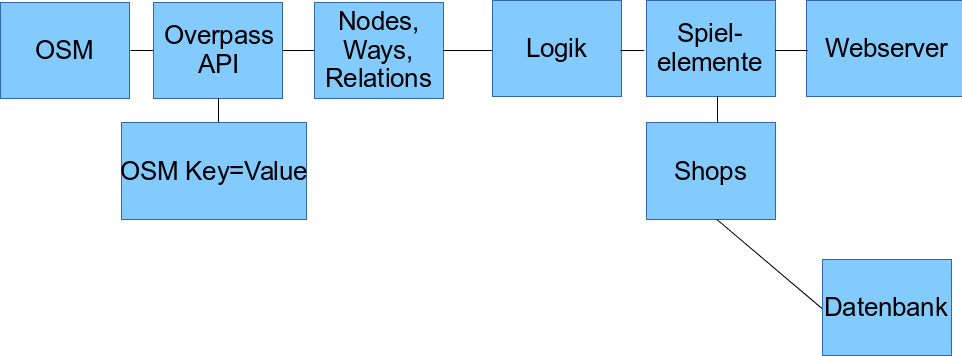
\includegraphics[width=140mm]{images/ch5_img01_framework_progress.png}
\caption{Prozess: Von OSM zum Spielelement}
\label{img:ch5_img01_framework_progress}
\end{center}
\end{figure}

\subsection*{OSM und Overpass API}

Zunächst steht zu Beginn des Prozess als Datengrundlage Openstreetmaps.
Die Daten werden allerdings nicht direkt von OSM über die OSM API abgerufen, sondern über Overpass. Das liegt daran, dass die OSM API selbst nur sehr rudimentäre Abfragen erlaubt.
Stattdessen wird die Overpass API verwendet, da diese geografische Abfragen erlaubt \cite{Meyer.2013}.
Diese Abfragen sind notwendig, um die zuvor deklarierte Anforderung, die Spielelemente basierend auf einem OSM key-value Paars zu bewerkstelligen. Darüber hinaus wird die Transformation der Relations und Ways in Nodes einfacher ermöglicht.
Durch die Verwendung der Overpass QL-Abfrage Sprache (OQL) ist es möglich sich nicht nur die jeweiligen Relations, Ways und Nodes eines tags zu erhalten, sondern auch zusätzlich alle rekursiv enthaltenen Elemente. Dies ermöglicht es den kompletten Datensatz mit einer Abfrage zu erhalten der für die spätere Transformation benötigt wird. Der Vorteil liegt darin, dass nicht mehrere Abfragen gestartet werden müssen und somit die Zeit bis alle Daten zur Verfügung stehen erheblich reduziert wird. Die Overpass API selbst bietet diverse Ausgabe Formate wie XML und JSON \cite{Olbricht.2014}. Für eine konkrete Umsetzung wurde sich bewusst für JSON entschieden, da zum einen die Performance bei der Verabreitung von JSON Dokumenten beachtlich höher ist im Vergleich zu XML Dokumenten \cite{Nurseitov.2009}. Zum anderen soll die Daten später als GeoJSON aufbereitet werden.
Der Aufruf der OverpassAPI erfolgt mittels einfacher REST-Abfrage:
\\\\
\url{http://overpass-api.de/api/interpreter?data=OQL_BEFEHL}
\\\\
Über den Parameter "data" wird der jeweilige OQL Befehl abgesetzt.
Für die Weiterverarbeitung der Daten wird im Anschluss das JSON Ergebnis vom Framework geparst und weiterverarbeitet.

\subsection*{Transformations Logik}

Die Transformation der Relations und Ways wird wie in Kapitel \ref{ch4:s:choosen_solution} umgesetzt. Eine Visualisierung ist in Abbildung \ref{img:ch5_img02_transform} zu sehen.

\begin{figure}[H]
\begin{center}
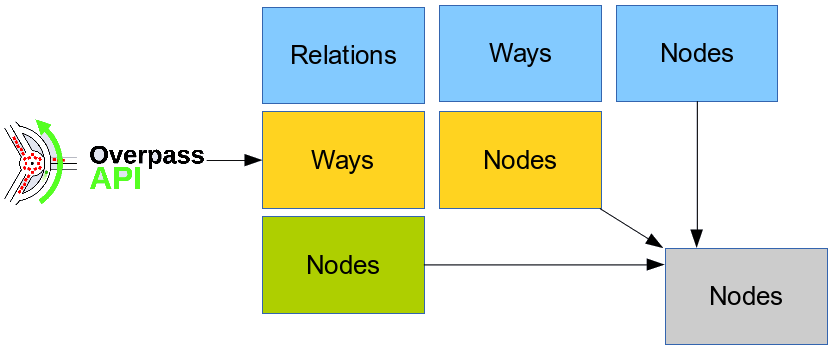
\includegraphics[width=140mm]{images/ch5_img02_transform.png}
\caption{Transformationsprozess: Relations, Ways, Nodes}
\label{img:ch5_img02_transform}
\end{center}
\end{figure}

Auf der linken Seite sind vertikal die Ausgangstypen angeordnet. Hierbei handelt es sich um die bereits angesprochenen Elemente Relations, Ways und Nodes. Im zweiten Schritt, nach dem Aufbereiten der Daten von der Overpass API wird wie folgt vorgegangen. Zunächst werden alle Relations behandelt, im Anschluss darauf die Ways und zum Schluss die Nodes. Die Idee dahinter ist es zunächst alle Ways und Nodes zu identifizieren welche direkt einer Relation angehören und keine separaten Spielelemente darstellen. Die Vorgehensweise ist damit begründet, dass durch die Reduzierung der Anfrage auf ein einzelnen Request die Rückgabe alle Nodes enthält. Sowohl die Nodes einer Relation, als auch die eines Ways, welche selbst nicht eigenständig sind. Daher müssen die Elemente Ebene für Ebene wie in der Abbildung zu sehen, abgearbeitet werden.
\\\\
Zunächst werden alle Relationen identifiziert. Für jede Relation werden nun die beinhalteten Ways und Nodes identifiziert. Diese wiederum werden dann als "gecalaimed" markiert. Relations selbst werden nicht rekursiv aufgelöst, da das Ziel nicht ist möglichst wenige Spielelemente zu haben, sondern Relationen zu transformieren. Sollten Relations mehreren Unterrelations haben so sollen diese als Eigenständige Elemente betrachtet werden. Sofern dieser Ansatz sich als Nachteilig in der Evaluation herausstellt muss er entsprechend modifiziert werden.
Für die jeweilige Iteration eines Relation Elements werden nun alle beteiligten Ways und Nodes zu einer Liste von Nodes zusammengefasst, Diese Liste wird wiederum durch das in Kapitel \ref{ch4:s:choosen_solution} beschriebene Verfahren einer Bounding Box dessen Mittelpunkt berechnet wird reduziert auf ein virtuelles Node, welches die Relation repräsentiert. Dieses virtuelle Node hat eine Koordinate, sowie eine ID welche eindeutig identifizierbar ist. Hierzu wird die Relations ID von OSM verwendet.

Im nächsten Schritt werden die Ways abgearbeitet. Bereits als "geclaimed" markierte Ways, die somit bereits in einer Relation enthalten sind, werden ignoriert. Alle anderen Ways werden entsprechend jeweils wiederum zu einer Liste von Nodes und anschließend zu einem virtuellen Node transformiert. Hierbei entsteht wieder eine Koordinate und als ID wird die OSM Way ID verwendet.

Die Elemente, welche direkt als Node zurückgegeben werden analog übernommen. Sie werden in Spielelemente, hier durch das graue Nodes Element symbolisiert, transferiert. Hierzu wird die Koordinate, sowie die OSM ID der Nodes übernommen.

Eine Problematiks tellt sich allerdings noch in der eindeutigen Identifizierung der virtuellen Nodes. Da diese von unterschiedlichen Elementen (Relatons, Ways, Nodes) abgeleitet wurden muss sichergesteltl werden, dass anhand der ID eine eindeutige OSM Zuordnung möglich ist.
Entweder es wird zusätzlich der abgeleitete typ des Spielelements explizit gespeichert oder aber, man transcodiert die Information mit in die ID.
Wenn man sich zunächst die OSM IDs für Nodes anschaut, stellt man fest, dass diese die 32bit signed Integer Grenze überschritten haben (Februar 2013). Im OSM Wiki wird daher empfohlen den Datentyp long zu verwenden, welcher in den Standard-Implementierungen ein 64bit Wert ist \cite{OSM.2013b}.
Eine Methode um den Typ des Spielelements zu übertragen könnte mit einer Bitmaske der ID funktionieren. Hierzu könnte man die den 2. und 3. Bit Bits des 64bit Wertes verwenden. Der 1. it wird nicht verwendet um negative Zahlen weiterhin zu erlauben. Der 2. Bit würde als Identifikator für Relations dienen und der 3. für Ways als Ursprungselement. Ein Beispiel für den transformierten Way mit der OSM ID 1 ist in Abbildung \ref{img:ch5_img03_bitmask} zu sehen.

\begin{figure}[H]
\begin{center}
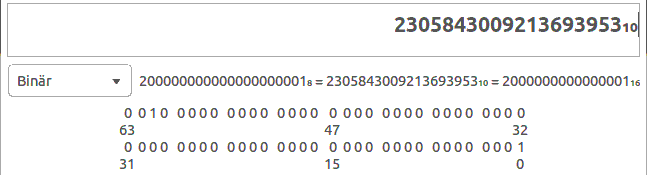
\includegraphics[width=120mm]{images/ch5_img03_bitmask.png}
\caption{OSM ID: Bitmaskenkodierung im 64bit long Wert}
\label{img:ch5_img03_bitmask}
\end{center}
\end{figure}


Wenn man die Reduzierung von 63bit (signed) auf 61bit(signed) mit der aktuellen Mapping Geschwindigkeit bei OSM vergleicht, so lässt sich feststellen, dass die Reduzierung um 2 bit aus Paradigmensicht zwar unsauber erscheint, aber eine Überschreitung der ID \begin{math}2^{61}\end{math} in ferner Zukunft liegt. Zudem könnte im Bedarfsfall wenn OSM auf 128bit IDs umsteigt die Bitmaske entsprechend angepasst werden.

\subsection*{Händler Integration}

Nachdem die virtuellen Nodes für die Spielelemente alle erstellt wurden, müssen die Elemente um die Händlern ergänzt werden. In Kapitel \ref{ch4:s:choosen_solution} wurde erläutert, dass die Händler nicht als aktives Spielzielelement verwendet werden sollen, sondern eine Integration der Händler und Dienstleister im Spiel als Repräsentation ihrer Selbst. Die Händler fungieren in diesem Zusammenhang als Anbieter für Items und andere Gegenstände. Für die spätere Darstellung auf der Karte müssen diese ebenfalls mit einer Koordinate versehen werden und separat behandelt werden. D.h. die Spielpunkte der Händler kommen stattdessen aus einer lokalen Datenbank. Dabei wird bewusst auf die Verwendung von OSM Als Basis verzichet. Zwar könnte man in einer erweiterten Version des Frameworks dem Nutzer unterstützen mit automatischen Vorschlägen basierend auf OSM, jedoch ist dies in der Grundfunktion nicht notwendig. Hier soll der Händler sich beliebig frei auf der Karte Positionieren können und entsprechende Parameter seines virtuellen Geschäfts festlegen. Im Anschluss soll er entsprechende Items in seinem virtuellen Shop hinterlegen können. Da die Items eventuell vom Händler gegen einen Betrag vom Spielleiter erkauft werden, hat der Spielleiter ein gewisses Interesse, dass er zum einen die Items im Spiel möglichst an die Spieler bringt, während er auf der anderen Seite das Spiel nicht in einen nicht balancierten Zustand bringt. D.h. dass eventuell zu viele Spieler durch die Nähe eines Händlers mit einem sehr nützlichen Item bevorzugt werden. Daher sollte es im Ermessen des Spielleiters liegen, dass dieser die Art und Verwendung der Items selbst definiert und entsprechende Vorschläge für die Händler parat hat. Dass der Händler selbst sich mit Spielmechaniken und Balancing auseinander setzt ist höchst unwahrscheinlich und würde auch nur zu extra Koordinationsaufwand führen. Daher ist es am sinnvollsten dem Händler gewisse Items mit standard Eigenschaften anzubieten, von denen er einen Typ selbst auswählt und eine entsprechende Menge seinem virtuellen Shop zuordnet.
Für die Itemtypen kann der Spielleiter aller Voraussicht nach auf gewisse Grunderfahrungen zurückgreifen. Darüber hinaus sollte das Framework ihm zu einem späteren Zeitpunkt in einer erweiterten Ausbauphase auch entsprechendes Feedback über die Verwendung und Nutzung der Items aufzeigen und der Spielleiter somit aufgrund dieser Information Rückschlüsse auf das Balancing machen kann.

\subsection*{Persistenz}

Ein wichtiger Aspekt des Frameworks stellt die Persistenz dar. Es müssen die Spielelemente, sowie der Spielzustand selbst gespeichert werden. Die Daten für die Spielelemente stammen aus OSM und von der lokalen Datenbank. Da die OSM Daten entsprechend transformiert werden stellt sich die Frage ob dieser Prozess beschleunigt werden kann, wenn die Daten entsprechend in der Datenbank lokal zwischengespeichert werden.
In Kapitel \ref{ch4:s:choosen_solution} ist bereits auf diesen Aspekt eingegangen worden. Die Problematik die sich durch eine Zwischenspeicherung stellt ist zum einen die Aktualisierung der Daten. Die lokalen Daten müssten mit einem Zeitstempel versehen werden und gehalten werden, bis diese "verfallen". Darüber hinaus müssten diese nach dem Verfallszeitpunkt entsprechend gelöscht oder aktualisiert werden oder belassen werden. Ein Caching kann hier Sinn sofern das Framework für ein Spiel mit einer kritischen Masse an Spielern verwendet wird. Allerdings ist eine Evalutation und Untersuchung des Frameworks auf Hochskalierbarkeit nicht Bestandteil der ersten Ausbaustufe. Ein weiterer Aspekt stellt die Datenmenge dar. Sofern im Framework alle jemals abgefragten OSM Daten in virtuellen Nodes/Spielelementen in der Datenbank hinterlegt werden ohne dass diese eine Zustandsveränderung erfahren haben ist dies zwar Modelltechnisch korrekt, allerdings aus Performance und Platzgründen nicht zu empfehlen. Speziell in der Hinsicht, dass das Framework dem Spielleiter so wenig Aufwand wie möglich machen soll, sollte verhindert werden, dass der Spielleiter sich um Datenbank und Speicherplatz Probleme kümmern muss. Ein gutes Beispiel hierfür stellt auch das OSM Projekt selbst dar. Die bekannte Kartendarstellung verwendet zur Anzeige entsprechende Tiles. Diese Tiles werden auf Basis der OSM Daten gerendert. Ein erster Ansatz wäre es alle Tiles entsprechen dzu Rendenr. Allerdings dauert der Renderprozess dann Tage und Aktualisierungen auf der Karte würden immer nur mit mehreren Tagen Verzögerung angezeigt. Hinzu kommt die Tatsache, dass nur ein Bruchteil der Kartendaten auch tatsächlich angeschaut wird (<2\% - OSM Quelle?). Daher werden die Karten-Bilddaten in Echtzeit gerendert und und nach einer gewissen Zeit wieder verworfen.
Daher ist es auch hier nicht sinnvoll alle Daten zu speichern sondern nur die Spielelemente mit denen ein Spieler aktiv interagiert hat.
Die Daten der Händler werden separat gespeichert. Sie befinden sich ebenfalls in einer Datenbank, besitzen allerdings im Vergleich zu den Spielelementen eine Persistenz unabhängig von ihrer Interaktion.


\subsection*{Schnittstellen}

Ein Framework benötigt entsprechende Schnittstellen über die es Funktionen und Daten nach Außen hin zur Verfügung stellt. Zunächst muss geklärt werden, wie die Daten verwendet werden sollen. Für das Beispiel-Spiel ist die Darstellung der Karte über eine Website vorgesehen. Unabhängig von der später verwendeten Technologie müssen in diesem Fall sowohl die Spielelemente, als auch die Händlerdaten vom Framework zur Verfügung gestellt werden.

Zur Verdeutlichung wird an dieser Stelle die Entscheidung für eine Technologie in Abbildung \ref{img:ch5_img04_interfaces} auf das nachfolgende Kapitel verlegt.

\begin{figure}[H]
\begin{center}
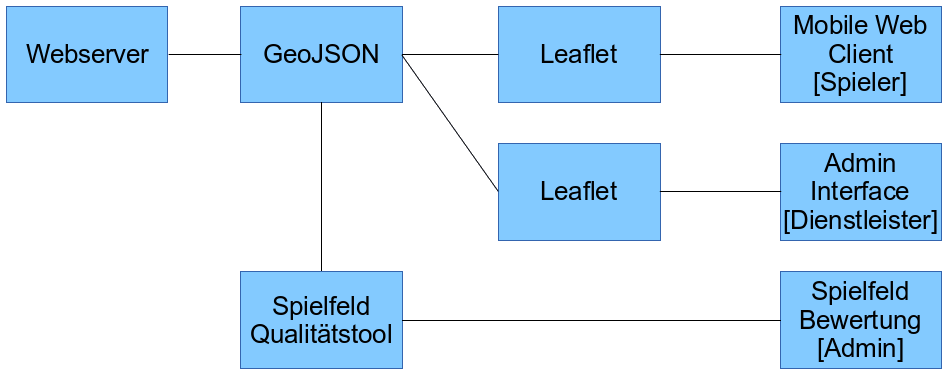
\includegraphics[width=140mm]{images/ch5_img04_interfaces.png}
\caption{Visualisierte Schnittstellen des Frameworks}
\label{img:ch5_img04_interfaces}
\end{center}
\end{figure}

Dadurch, dass das Framework die Daten von OSM/Overpass als JSON erhält und das Format bestens geeignet ist für den Austausch, da eine Vielzahl der aktuellen Frameworks und Tools dieses unterstützen ist die Wahl auf den Export der Spielelemente und Händlerdaten auf GeoJSON gefallen. Während das offene Format WKT für die reine Repräsentation von Geodaten dient \cite{Stolze.2003}, bietet das GeoJSON FOrmat zusätzlich die Möglichkeit entsprechende Properties an ein Geo Objekt zu speichern \cite{Butler.2008}. Über diese kann wiederum das Framework Informationen wie z.B. die codierte OSM ID und Informationen zum Spielelement übertragen.
\\\\
Generell werden die Informationen des Frameworks für drei verschiedene Module benötigt.
Zunächst einmal gibt es den Spielclient bzw. dessen Oberfläche. Dieser benötigt die Daten für das Staging des Spiels selbst.
Über die Spieloberfläche interagiert der Spieler mit dem Spiel. Er Sieht die aktuelle Karte, sowie die darauf platzierten Objekte. In diesem Fall sind dies die Spielelemente sowie die einzelnen Händler. Die Spielelemente selbst stellen im Beispielspiel die sogenannten Prestige Flaggen dar.
Ein weiteres Moduls stellt die Administartionsoberfläche dar. DIese dient dazu dem Spielleiter sowie dem jeweiligen Händler eine Konfiguration des Spiels vorzunehmen. Im Detail kann der Spielleiter die entsprechenden Spielitems definieren, neue Händler anlegen und diese auf der Karte positionieren. Der Händler kann seine Metadaten pflegen und entsprechende Items, welche er in seinem virtuellen Laden anbieten möchte selektieren und anbieten. Bei Fehlern oder Aktualisierungen kann der jeweilige Administrator (Spieleiter oder Händler) diese problemlos anpassen. Für die Positionierung der virtuellen Läden auf der Karte wird ebenfalls analog zum Spielfeld eine GeoJSON Schnittstelle zum Einsatz kommen.
Das letzte Modul stellt die Evaluierung der Spielfelder dar. Hier wird dem Spielleiter durch die Verwendung der gleichen Schnittstelle, wie für die Aufbereitung des Spielfeldes, die Möglichkeit geboten Daten in ein entsprechendes Evaluationstool mit entsprechendem Algorithmus  zu importieren. Dieses Tool wird entsprechend in Kapitel \ref{ch:CH6_qualtiy_of_gameboards} in vorgestellt. Über dieses wird das ideale Key-Value Paar für die OSM Tag Selektion der Daten evaluiert. Dies soll dem Spielleiter die Möglichkeit einer Objektiven Bewertung der Spielfelder ermöglichen.

\subsection*{Darstellung}

Da das Framework für ortsbezogene Spiele verwendet werden soll, ist es daher unerlässlich dem Spieler, sowie den Administratoren eine entsprechende Visualisierung zu bieten. Zunächst gibt es das Spielfeld. Das Spielfeld verwendet im Hintergrund Kartenmaterial von OSM, auf das die einzelnen Elemente platziert werden. Die Karte selbst wird initial auf die (GPS-)Korrdinaten der Spielerposition zentriert. Dadurch ist es dem Spieler möglich sich direkt von seiner Position aus zu Orientieren. Die auf der Karte eingezeichneten Eleemente wie Flaggen und Händler kann der Spieler somit problemlos identifizieren und zu Fuß aufsuchen. In Abbildung \ref{img:ch5_img05_dialog} ist ein Mockup der Kartenoberfläche zu sehen. Je nach Flaggestatus werden die Flaggen unterschiedlich farbig dargestellt. Das Ziel ist es Neutrale Flaggen grau, feindliche Rot und eigene grün darzustellen. Damit erhält der Spieler automatisch einen Überblick über die Situation und kann auch durch das Herauszoomen der Karte seine weiteren Spielzüge entsprechend planen.
Über die Elemente hinaus werden dem Spieler sein aktueller Punktestand. Dieser wird im Beispielspiel durch das einfache Addieren der Prestige der Flaggen die im Spielerbesitz sind berechnet. Des weiteren wird dem Spieler eine Auswahl für sein Inventar angezeigt werden. Über dieses kann er nicht nur sich alle Items in seinem Besitz anzeigen lassen, sondern auch diese verwenden und in einem späteren Ausbau des Frameworks Items mit anderen Spielern tauschen.
Sofern der Spieler mit einer Flagge interagiert, wird ihm die aktuelle Prestigezahl der Flagge angezeigt. Je nachdem ob ihm die Flagge bereits gehört oder diese einem fremden Spieler angehörig ist, kann der Spieler diese "angreifen". Durch den Angriff werden die Aktionspunkte des Spielers auf die Flagge transferiert. Ist die Flagge im Besitzt eines anderen Spielers so sieht der Spieler dies durch die aktuelle Farbgebung und kann durch den Einsatz seiner Aktionspunkte die Prestigezahl reduzieren, was direkt angezeigt wird. Für die Interaktion mit Händlern, steht dem Spieler ebenfalls ein Menü zur Verfügung, sobald er auf einen der Händler klickt. Danach öffnet sich ein Menü über das der Spieler eine Übersicht der verfügbarne Items sowie deren Spielpreise erhält. Sollte der Händler darüber hinaus Items wie in Kapitel \ref{ch4:s:choosen_solution} angedeutet mit Coupons arbeiten, so kann der Spieler diesen an gegebener Stelle eingeben.

\begin{figure}[H]
\begin{center}
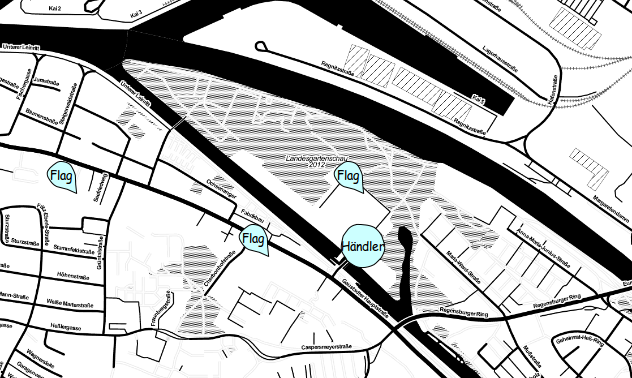
\includegraphics[width=140mm]{images/ch5_img05_dialog.png}
\caption{Spielfeld Mockup}
\label{img:ch5_img05_dialog}
\end{center}
\end{figure}

Der Administrationsbereich für den Spielleiter und den Händler arbeitet separat vom Spielfeld.
Je nachdem, ob Items oder Händler in das System gepflegt werden sollen, wird der Benutzer mit einer Liste präsentiert.
Im Fall der Items, erhält der Benutzer eine Übersicht über alle Items die dem Spiel zur Verfügung stehen. Hierbei handelt es sich allerdings nicht um Itemtypen sondern direkt um die instantiierten Items selbst. Die Idee dahinter ist es, dem Spiel die Möglichkeit zu bieten auch einzigartige Items zu enthalten und sicherzustellen, dass ein Item jeweils auch immer als solches im System behandelt wird. Über die Liste gibt es die Option die bestehenden Items zu modifizieren oder zu entfernen. Neue Items können übe reine Schaltfläche entsprechend angelegt werden. Dabei wird dem Benutzer eine entsprechende Oberfläche präsentiert und über Metadaten das Item genauer spezifiziert. Beispielsweise der Name, Itemtyp und der dafür  zu zahlende Preis.
\\\\
Möchte der Benutzer dahingegen Händler pflegen, so erhält er zunächst analog zu den Items eine Übersicht der einzelnen Händler.
Diese kann er analog zu den Items entsprechend modifizieren und löschen. Auch das Anlegen eines neuen Händlers ist analog zu den Items. Der Unterschied liegt jedoch drin, dass es sich bei den Händlern nicht um einfache Formularfelde rhandelt, sondern auch zusätzlich eine Georepräsentation stattfinden muss. D.h. es muss die Position des Händlers auf einer Karte erfolgen. Hierzu wird eine Art "Picker" verwendet. Auf einer OSM Karte soll der Benutzer die Position des Händlers definieren. Für eine Korrektur der Position reicht es aus, wenn der Benutzer einfach den Marker auf der Karte mit der Maus ergreift und per drag n drop auf seine neue Position bewegt.

%%\subsection*{Sonstige Funktionalitäten}


\subsection*{Technischer Entwurf}

Nachdem die Anforderungen beschrieben wurden, muss der Softwareteschnische Entwurf konkretisiert werden.
Um die Software entsprechend abzubilden zu können muss zunächst ein Modell entworfen werden, welche die Software abbildet. Die Prozesse des Frameworks wurden bereits in Abbildung \ref{img:ch5_img01_framework_progress} sowie \ref{img:ch5_img04_interfaces} visualisiert.

Zu Beginn einer Systementwicklung müssen die Usecases und die beteiligten Akteure identifiziert werden.
Hierfür wird zu Beginn überlegt, welche Personen Zugang zum System haben und welche Aufgaben diese am System erfüllen werden.
Dadurch wird sichergestellt, dass alle Aspekte behandelt werden, nicht nur die im initialen Lösungsansatz. Diese sind wichtig für den späteren Entwurf des Systems, sowie deren Umsetzung.
Die Usecases lassen sich als Diagramm wie in Abbildung \ref{img:ch5_img06_usecases} sichtbar definieren.



\begin{figure}[H]
\begin{center}
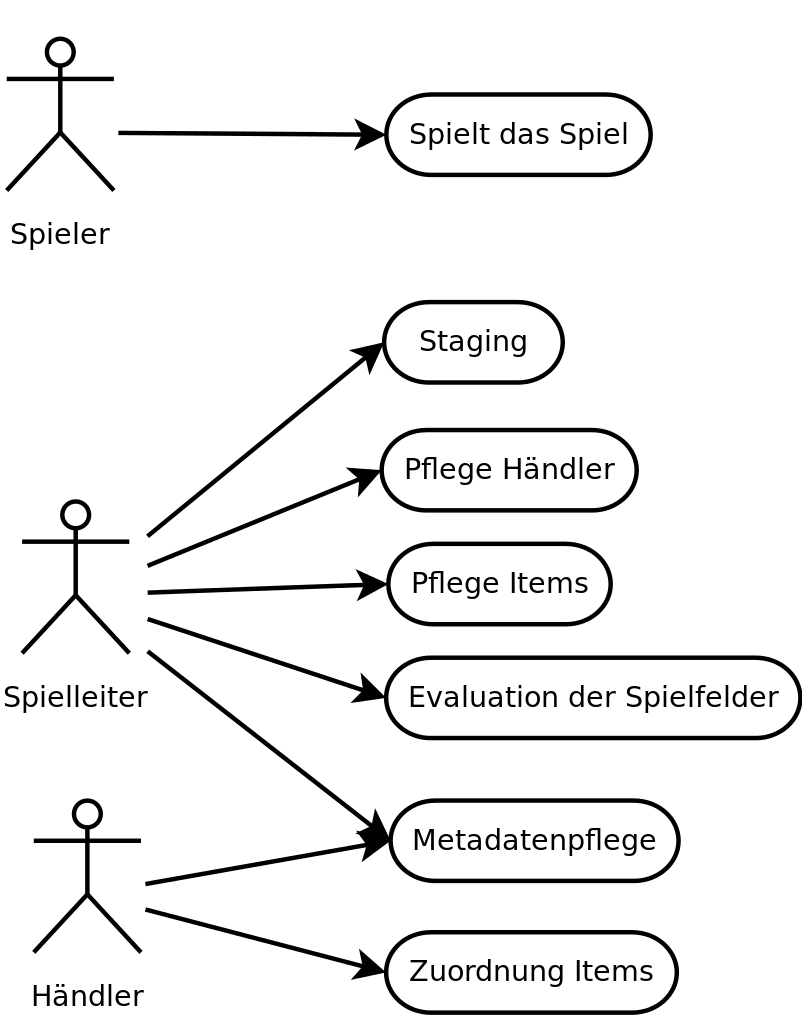
\includegraphics[width=100mm]{images/ch5_img06_usecases.png}
\caption{Usecase Diagramm}
\label{img:ch5_img06_usecases}
\end{center}
\end{figure}

Zunächst lässt sich feststellen, dass es drei Akteure gibt.
Diese decken sich soweit mit dem Lösungsansatz.
Der Spiele hat das Ziel das Spiel zu spielen. Der Spielleiter hingegen sieht es vor entsprechend das Staging des Spiels mit dem Framework zu bewerkstelligen.
Hier muss er die Händler als auch Items pflegen. Darüber hinaus teilt er sich mit dem Händler die Metadatenpflege, da je nach Situation der Spielleiter mehr oder weniger in die individuelle Pflege der Händlerdaten eingebunden ist. Der Händler möchte zusätzlich seine Items, die er vom Spielleiter zugewiesen bekommen hat entsprechend auf seine virtuellen Läden verteilen. In der Grundfunktion des Framesworks sind nur diese Benutzer vorgesehen. In einem Ausbau des Frameworks macht es Sinn explizite Nutzerrollen einzuführen um eine detailliertere Rechtezuweisung zu ermöglichen.
\\\\
Durch die Verwendung einer objektorientierten Programmiersprache ist es notwendig entsprechende Klassen zu definieren.
Diese dienen dazu, Objekte abzuleiten und die jeweiligen Methoden von diesen zu nutzen.
Es muss sichergestellt werden, dass die Beziehungen zwischen den Klassen modular sind, damit ein einfacher Zugriff und eine Austauschbarkeit gegeben ist.
Um ein Einblick in die Struktur des Frameworks zu erhalten wird in diesem Abschnitt kurz auf die wichtigsten Aspekte eingegangen.


\begin{figure}[H]
\begin{center}
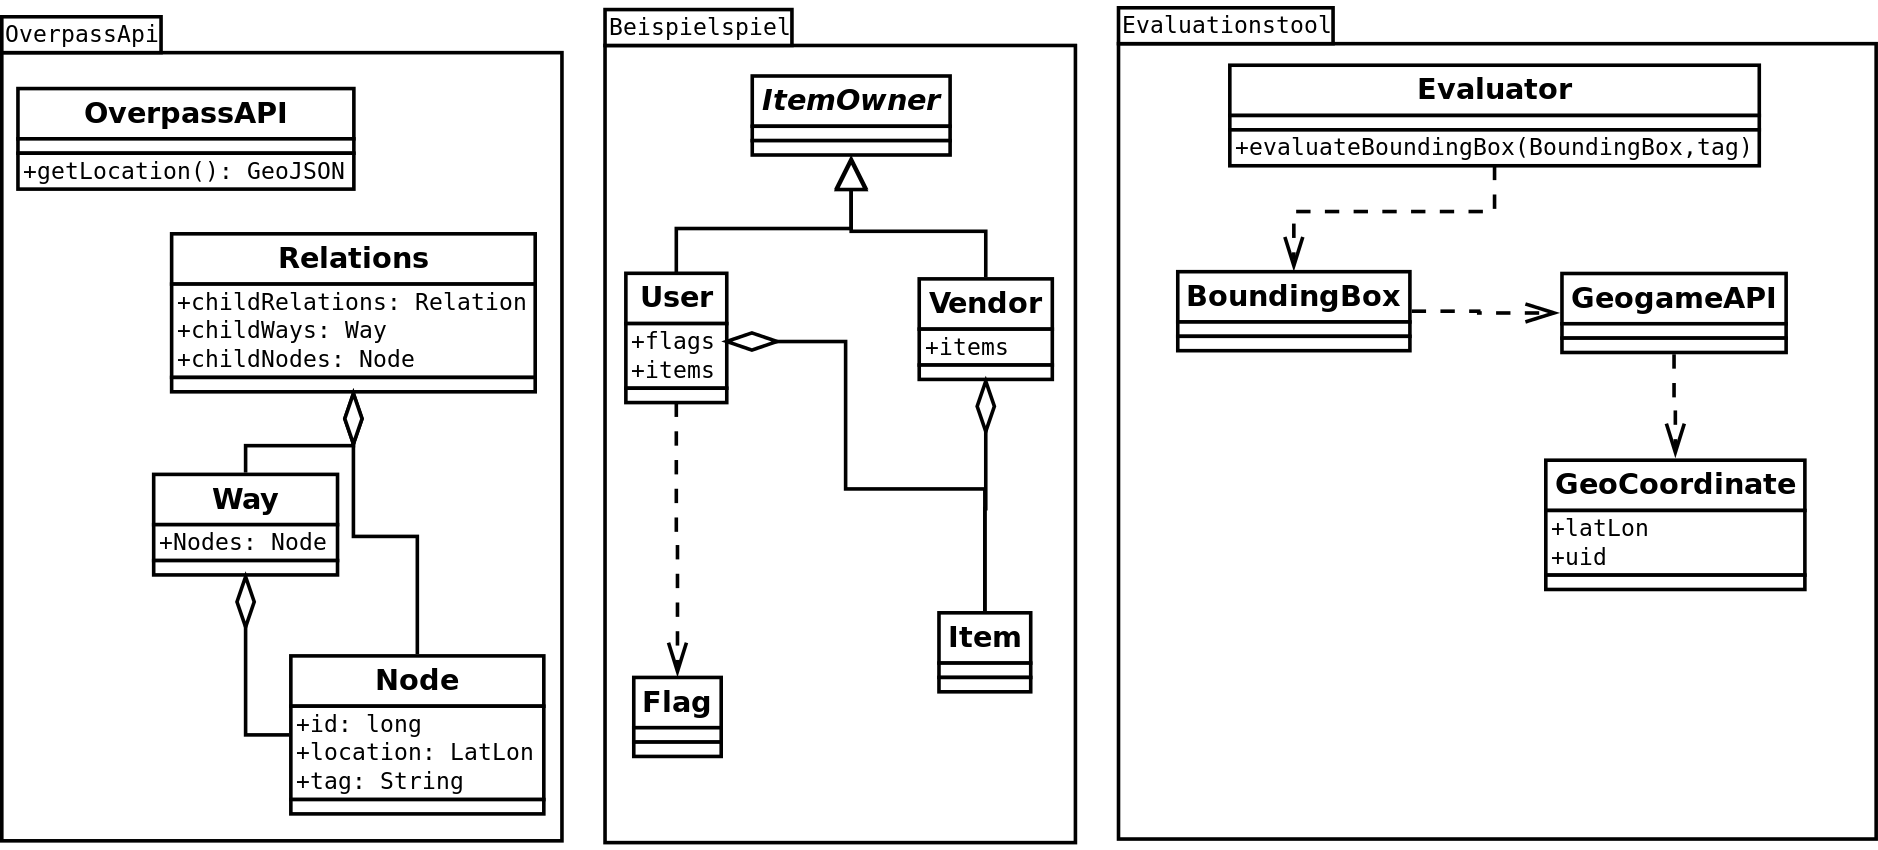
\includegraphics[width=150mm]{images/ch5_img07_classes.png}
\caption{Vereinfachtes Klassen Diagramm}
\label{img:ch5_img07_classes}
\end{center}
\end{figure}

In Abbildung \ref{img:ch5_img07_classes} ist ein vereinfachtes Klassendiagramm des Frameworks zu sehen. Das Framework als solches besteht aus drei Modulen. Zunächst gibt es den Bereich \textit{OverpassApi}. Hierbei handelt es sich nicht um die OverpassApi selbst, da Overpass selbst nur eine Webschnittstelle ist, sondern um die Implementierung einer entsprechenden Schnittstelle im Framework selbst, welches das Ergebnis der OverpassApi im Web transferiert auf die einzelnen Elemente Relations, Ways und Nodes. Diese werden wiederum durch den bereits beschriebenen Ansatz entsprechend transformiert in dem eine umcodierung in virtuelle Nodes erfolgt. Im gleichen Zug wird überprüft, ob es persistierte Daten für die virtuellen Nodes in der lokalen Datenbank gibt. Ist dem der Fall, so werden die virtuellen Nodes um die entsprechenden Properties ergänzt und anschließend als JSON bzw. GeoJSON gerendert.
Im Anschluss werden diese über die Webschnittstelle des eigenen Frameworks ausgegeben.
Für die Händler gibt es eine separate Schnittstelle im Framework, welche analog zur Overpass Implementierung fungiert, aber hierbei nicht die Daten von extern (OSM/Overpass) bezieht, sondern direkt in der fertigen Form aus der lokalen Datenbank auslesen kann. Hierbei ist zudem auch keine entsprechende Transformation notwendig, sondern diese liegen bereits als fertige Nodes vor. Dies ist möglich, da jeder Händler nur als einziger Punkt im Spiel repräsentiert wird.
\\\\
Das nächste Modul ist das \textit{Beispielspiel}. Das Beispielspiel selbst wurde einfach gehalten, da es zum einen als Proof of Conecept des Frameworks dienen soll, zum anderen der Fokus auf die Verteilung der Spielelemente auf dem Spielbrett untersucht werden soll.
Generell gibt es 4 Objekte. \textit{Spieler}, \textit{Händler}, \textit{Flaggen} und \textit{Items}.
Spieler und Händler stehen in einer polymorphen Verbindung zu Item. Ausgelöst, leiten beide Klassen von einer abstrakten Klasse \textit{ItemOwner} ab, welche entsprechende Methoden vorhält die für die Interaktion als ItemOwner essentiell sind. Beispielsweise der Verkauf oder die Benutzung eines Items. Ein Item kann nur einem Spieler oder einem Händler angehören, niemals aber beiden gleichzeitig. Des weiteren gibt es auch die Möglichkeit, dass ein Item ohne ItemOwner existiert. Ein Beispiel könnte es sein, dass der Spielleiter für ein Event bestimmte Items auf der Karte ablegt oder lokale zwei Spieler Items manuell tauschen möchten.
\\\\
Das letzte Modul stellt das sogenannte \textit{Evalutationstool} dar.
Mit diesem sollen die erzeugten Spielfelder analysiert und bewertet werden. Eine genauere Erläuterung ist in Kapitel \ref{ch:CH6_qualtiy_of_gameboards} zu finden.
Das Evaluationstool gereift zunächst auf die GeoJSON Schnittstelle des Frameworks zu. Dieses liefert bei entsprechender Abfrage mittels Bounding Box und entsprechendem OSM Tags die Spielelemente zurück. Die Boundingbox wird auf Basis einer initialen Koordinate berechnet. Somit kann der Spielleiter einfach zwei Koordinaten definieren zu denen er gerne eine entsprechende Auswertung interessanter Tags erhalten möchte. Das Evaluationstool startet im Anschluss den Vorgang und wandelt die Spielelemente in vereinfachte Objekte mit ID und Geo-Kooridnaten um. Diese wiederum werden der jeweiligen Evaluationsmethode als Liste übergeben und deren Rückgabewert beschreibt die Kombination aus Boundingbox und OSM Tag.

\subsubsection*{Datenbank}

Aufgrund der vorherigen Analysen wird normalerweise ein Enitity Relationship Model (ERM) erstellt. Allerdings soll der Einsatz eines Webframeworks erfolgen welches ein mindestens ein Objektrelationales Mapping unterstützt und somit die Manuelle Erstellung der Datenbankstruktur nicht mehr vorgesehen ist. Dies wird unter der Annahme gemacht, dass das Framework später im Produktiv Betrieb für die Datenspeicherung optional auf eine NoSQL Lösung umgestellt werden kann. Diese bieten eine bessere Performance bei einfachen Abfragen.
Dies geschieht auch vor dem Hintergrund den in der Literatur häufig kritisierten Mismatch zwischen Objektorientierter Programmierung und der Verwendung von Relationalen Datenbanken um Objekte welche von Klassen abgeleitet wurden zu speichern \cite{Cattell.1991}.

Die geringe Verbreitung der objektorientierten Datenbanken liegt darin, dass nicht
versucht wurde die bestehenden Datenbanken zu ersetzten. Viel mehr sind die bereits existierenden Datenbanken in Unternehmen nicht in neue objektorientierte Datenbanken transferiert worden. Der Grund hierfür liegt in den historisch gewachsenen Applikationen und Datenbanken, dessen Umstellung einen sehr hohen Aufwand und Kosten darstellen würde \cite{Burleson.1994}.

Ein weiter Aspekt ist die Tatsache, dass die objektorientierten Datenbanken nicht in jedem Aspekt
besser sind als relationale Datenbanken. Es gibt Situationen in denen haben Objektorientierte
Datenbank Management Systeme klare Vorteile gegenüber den relationalen Datenbanken besitzen.
Die Objektorientierten Datenbanken spielen Ihre Vorteile speziell bei der Abbildung
von Beziehungen von Objekten untereinander aus. Nicht nur bei Vererbungen sondern auch wenn
die Objekte diverse Methoden besitzen. Bei einer Sequentiellen Abfrage mehrerer Datensätze sind
jedoch die relationalen im Vorteil \cite{Van.2006}. Hier ist es notwendig den Zweck der zu speichernden Daten bzw. deren Verwendung zu untersuchen. Je nachdem kann der Einsatz von objektorientierten Datenbanken oder relationalen Datenbanken Sinn machen.

Vergleicht man die Verbreitung von objektorientierten Datenbanken in gewissen Einsatzgebieten, so lässt sich feststellen, dass diese trotz der in Summe geringen Verbreitung ein berechtigtes Dasein haben. Speziell in Geoinformationssystemen spielen objektorientierte Datenbank Management Systeme ein wichtige Rolle,\cite{Brinkhoff.2005} da Sie deutlich einfacher ermöglichen komplexe Verbindungen zwischen den unterschiedlichen Objekten herzustellen und eine Veränderung dieser Beziehungen in einem Bruchteil der Zeit ermöglichen, welcher eine relationale Datenbank dafür aufwenden müsste. Die umfangreiche Literatur zum Thema Geoinformationsysteme gibt einen Ausblick für Möglichkeiten sich durch die Nutzung dieser ergeben können.

\subsection*{Weitere Aspekte}

Ein weiterer Aspekt stellt die Optimierung der Anfragen an die Overpass Api Schnittstelle des Frameworks seitens des Spielfeldes dar. In der Grundvariante des Frameworks, stellt das Spielfeld jeweils eine Anfrage als Bounding Box an die Schnittstelle um die aktuellen Spielelemente für den jeweiligen Kartenausschnitt zu erhalten. Eine Optimierung dessen wäre es mit dynamischen erweiterten gecachten Bounding Boxen zu arbeiten. Das bedeutet, dass bei einer Abfrage zunächst die Boundingbox am Rand um jeweils 30\% erweitert wird. Die zusätzlichen abgefragten Spielelemente werden allerdings nicht direkt angezeigt. Bewegt der Spieler nun das Spielfeld wird überprüft ob der aktuelle Kartenausschnitt sich noch innerhalb der dynamisch erweiterten Bounding Box befindet. Ist dies der Fall, so spart sich der das Spiel einen zweiten Request. Dies hat zweierlei Vorteile der erste stellt eine Reduzierung der HTTP Request auf der Clientseite dar. Speziell bei ortsbezogenen Spielen ist der Empfang beim Spielen öfters eingeschränkt und nur GPRS oder EDGE seitens Mobilfunkanbieter verfügbar. Durch die Reduzierung der Reuqests wird die Spielperformance verbessert. Ein anderer Aspekt ist die Reduzierung der Anfragen auf der Server Seite. Es verbessert deutlich die Skalierbarkeit und ermöglicht somit mehr Spieler mit einem einzigen Server bedienen zu können.

%% performance messungen?

\section{Bewertung der Technologien und Werkzeuge}

Nachdem der Softwaretechnische Entwurf erstellt wurde, muss untersucht werden welche Technologien und Werkzeuge für die Umsetzung des Frameworks am besten geeignet sind.
Zunächst stellt sich die Frage in welcher Programmiersprache das Framework umgesetzt werden soll. Diese Frage lässt sich anhand der Anforderungen eingrenzen. Zunächst muss eine Website erstellt werden, welche ein Staging des Beispielspiel erlaubt und gleichzeitig die Spieldaten über eine Webschnittstelle exportieren kann. Hiermit lässt die Auswahl auf entsprechende Sprachen reduzieren, welche eine Erstellung dynamischer Webseiten erlauben.
Die nachfolgende Aufzählung nennt die aktuell verbreitetsten Sprachen \cite{WWWtechs.2014, Deitel.2008}:

\begin{itemize}
\item PHP (81.8\%)
\item ASP.NET (17.8\%)
\item Java (2.7\%)
\item ColdFusion (0.8\%)
\item Perl (0.6\%)
\item Ruby (0.5\%)
\item Python (0.2\%)
\item JavaScript (0.1\%)
\end{itemize}

Das Framework kann auf allen der genannten Sprachen umgesetzt werden.
Das Ziel ist es aber zum bevorzugt auf OpenSource Technologien zurückzugreifen, da diese ohne Lizenzkosten sind und meist guter Dokumentation bieten können. Damit fallen ASP.NET und ColdFusion aus der engeren Auswahl. Ein weiteres Kriterium stellt die Verwendung eines Web Frameworks dar. Ziel ist es das Framework zu implementieren und den Aufwand für andere Aspekte auf einem Minimum zu halten. Darüber hinaus reduzieren Web Frameworks auch die Gefahren im Hinblick auf Sicherheit \cite{Livshits.2007} und reduzieren den Implementierungsaufwand \cite{Schwabe.2001}. Für die restlichen Sprachen gibt es eine Vielzahl an entsprechender Web Frameworks \cite{Weinberger.2011}. Eine komplette Analyse über alle Sprachen hinweg, sowie deren Vor- und Nachteile ist nicht Bestandteil der Arbeit, daher wird ein Framework ausgewählt, welches dem Autor vertraut ist und eine möglichst effiziente und schnelle Umsetzung des Frameworks ermöglicht.
\\\\
In diesem Fall wurde sich daher für 'Ruby on Rails' entschieden, einem Webframework welches auf der Sprache Ruby basiert. Ruby bietet darüber hinaus eine Paketverwaltung analog zu den bekannten Paketverwaltungsystemem in etablierten Linux Distributionen \cite{Bachle.2007}. Durch eine Versionskoppelung der Pakete kann sichergestellt werden, dass ein Projekt problemlos auf allen Rechnern problemlos funktioniert, da fehlende Bibliotheken mit einem Befehl problemlos nachgeladen werden.
Ein weiterer Vorteil ist die feste Verwendung des Model View Controller-Patterns \cite{Tate.2006}. Durch dieses wird sichergestellt, dass das Modell komplett unabhängig von der Darstellung ist. Dies ist auch für das Game Framework wichtig. Speziell um konkrete Funktionen über Schnittstellen über und Dialoge zur Verfügung zu stellen. Allerdings ist zu beachten, das es sich in Webframeworks, in diesem Fall auch bei Rails um eine abgewandelte Form des MVC namens \textit{Model2} handelt \cite{Qiuhui.2002}. Der Controller wird mit dem Seitenaufruf angestoßen und interagiert mit dem Model. Im Anschluss verwendet der View die Ergebnisse/Daten des Controllers und rendert entsprechend die Webseite.
\\\\
Nachdem die Wahl des Webframeworks auf Ruby on Rails gefallen ist wurden entsprechende Bibliotheken für die Verwendung gesucht, welche Funktionen die für das Framework benötigt werden.
Die Vorteile fertiger Bibliotheken liegen darin, dass der Entwickler selbst nciht nur Zeit bei der Entwicklung spart, sondern auch durch die Reduzierung seines Codeumfangs auch eine Reduzierung von möglichen Fehlerquellen erreicht.

Modere Bibliotheken wie JQuery für JavaScript und Compass für Sass bzw. CSS werden mit Rails direkt unterstützt. Auch die Unterstützung von Coffee Script und Sass sind bereits integriert.

Das Game Framework muss auf auf spatiale Operationen zurückgreifen. Hierfür wird auf das Gem 'rgeo' zurückegriffen werden. Es handelt sich dabei um eine weit verbreitete Bibliothek die nicht nur mit geografischen Objekten umgehen kann, sondern auch direkt eine Anbindung von GIS-Datenbanken wie PostGIS, Spatialite und MySQL-Sptial erlaubt.\footnote{\url{http://dazuma.github.io/rgeo/}}

Ein weiterer Aspekt stellt die Kartendarstellung dar. Für die Kartendarstellung selbst gibt es mehrere Ansätze. Die am weitesten verbreiteten sind die Google Maps API, Openlayers und leaflet \cite{Derrough.2013}. Mit der Google Maps API kann man zwar die Openstreetmap Tiles als Layer laden, jedoch sind der kommerziellen Nutzung gewsse Einschränkungen unterworfen und der Quellcode nicht frei verfügbar. Da sich ein potentieller Spielleiter nicht mit den rechtlichen Problematiken und Lizenzvereinbarungen auseinander setzten sollte sollte diese vorzugsweise vermieden werden. Openlayers hat im Vergleich zu Leaflet eine längere Versionsgeschichte \cite{Ohloh.2014}. Und bietet deutlich mehr Funktionen. Allerdings ist OpenLayers mit 800KB deutlich größer wie Leaflet mit 120KB. Da es das Ziel ist, das Framework speziell auch im Zusammenhang mit Smartphones zu nutzen ist es wichtig, dass nicht nur die Dateigröße minimal ist, sondern auch eine möglichst gute Funktionsweise auf Smartphones sichergestellt wird. Hier ist Leaflet deutlich moderner und besser angepasst. Beide Bibliotheken unterstützen GeoJSON und ermöglichen somit die einfache Einbindung von Geo-Objekten. Die Entscheidung aufgrund der Anforderungen und ausreichenden Reife auf Leaflet. Auch für dieses gibt es bereits für Ruby ein entsprechendes Gem, welches Leaflet direkt für Rails integriert 'leaflet-rails'.

Neben der Kartendarstellung ist es auch wichtig, alle Spieler einzeln zu identifizieren und für jeden Spieler eine eigene "Spielsession" zu haben. Für die Benutzerverwaltung gibt es für Rails ebenfalls bereits fertige Lösungen. Diese kann man entsprechend für seine Bedürfnisse erweitern, muss trotz allem nicht komplett die Logik und Datenbankzugriffe für das Erstellen, Anlegen und Ändern von Benutzerdaten kümmern. Auch Funktionen, wie das zurücksetzten eines Passworts sind bereits integriert. An dieser Stelle wurde sich für das Gem 'Clearance' entschieden, da dies ausgereift ist und eine einfache Anpassung der Seitenbenutzer um zusätzliche Attribute ermöglicht, welche im Zuge des Frameworks entsprechend hinterlegt werden sollen.

Für die Schnittstellen welche das Gameframework anbieten soll, werden keine explizite Bibliotheken benötigt. Rails bietet automatisch die Möglichkeit für bestimmte Routen die passenden Dateiformate zu hinterlegen. Bei Routen handelt es sich bei Rails um Seitenpfade. Durch das Anlegen der Route '/flag/show/{id}' wird nach dem Aufruf des FlagControllers mit der Methode show die View show aufgerufen. Durch die Defaulteinstellung werden automatisch zuerst die html Files gerendert sofern der Request nichts anderes Fordert. Der View show.html.erb erhält somit nach dem Aufruf der show Methode ein entsprechendes Objekt mit der angegeben Id aus der Datenbank zurück. Möchte man allerdings das Element nicht als Webseite darstellen sondern als JSON Objekt, so legt man lediglcih eine entsprechende show.json.erb Datei an und kann direkt über die vorhandene JSON Bibliothek das Ibjekt entsprechend als JSON serialisieren.
Hier zeigt sich die Flexibilität und Einfachheit die sich durch die Kombination von Ruby und Rails ergibt. Dies macht das Webframework ideal für die Nutzung mit dem zu erstellendem Game Framework.

Für die Erstellung des Quellcodes kommen entsprechende IDE zum Einsatz sowie eine Softwareversionskontrolle. Dies ist hilfreich um durch die die Verwendung von Code Snippets sowie einer visualisierte Fehler-Erkennung und Lösung sicherzustellen.
Für das Schreiben des Java-Quellcodes des Evaluationstools wurde auf Eclipse zurückgegriffen. Eclipse ist ein bewärtes Tool und dem Autor bestens vertraut und  biete auch eine ausreichende Modularität durch die Installation von Erweiterungen über eine integrierte Verwaltung.
Für die Entwicklung des Ruby on Rails-Codes wurde der grafische Text-Editor Geany verwendet. Da ein reiner Textdeitor mit Syntax Highlighting und Code Completion keine Debbing Möglichkeitne bietet wurde auf spezielle Rails Gems zurückgegriffen.
Zunächst einmal wurde das bewerte 'Pry' Gem verwendet um ein einfaches Binding an entsprechender Code Stelle zu ermöglichen. Eine Parallele Rails Console ermöglicht dase das Überprüfen von entsprechender Active Record Abfragen, wie z.B. das Erfassen aller Punkte eines Spielers für die Status Übersicht. Für das direkte Debuggen von Fehlern zur Laufzeit  wurde das Gem 'better\_errors' in Verbindung mit 'binding\_of\_caller' verwendet. DIes ermöglicht es quasi Analog zum Debugmodus in Eclipse direkt an der Stelle an der ein unbehandelter Fehler auftritt in den Code einzusteigen. Das bedeutet es kann nicht nur einfach untersucht werden, an welcher Stelle und mit welchen Werten der Fehler auftritt, sondern direkt dort an der Stelle mit einer interaktiven Konsole aktiv debuggt werden. Eine Darstellung ist in Abbildung \ref{img:ch5_img08_livebinding} zu sehen. Dadurch ist es möglich ohne den Rails Prozess zu stoppen direkt hintereinander diverse Befehle zu testen und somit schneller die Ursache des Fehlers aufzufinden. Dies war vor allem im Zusammenhand der in Kapitel \ref{ch5:s:Implementierung} erläuterten Probleme bei der Entwicklung besonders hilfreich.

\begin{figure}[H]
\begin{center}
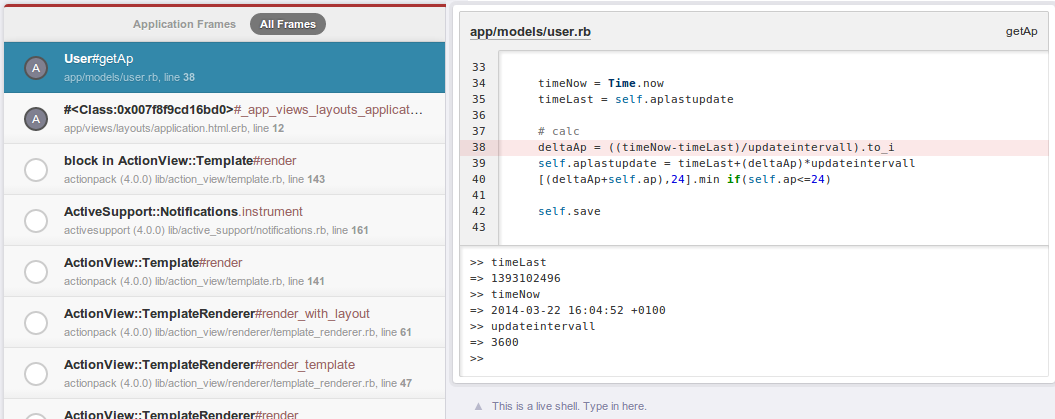
\includegraphics[width=155mm]{images/ch5_img08_livebinding.png}
\caption{Interaktives Debugging mit 'better\_errors' und 'binding\_of\_caller'}
\label{img:ch5_img08_livebinding}
\end{center}
\end{figure}

Für die Entwicklung von Software ist es essentiell beliebig den Code wiederherstellen zu können und einfach neue Funktionen auszuprobieren. Diese Anforderung bedienen Software Systeme zur Versionsverwaltung. 
Die Auswahl wurde auf ein Open-Source System gelegt. Am weitesten verbreitet sind zur Zeit Subversion und Git. Letzteres bietet Möglichkeit einer nicht linearen Entwicklung \cite{Bird.2009}.
Die Wahl fiel speziell auf Subversion, da es im Gegenzug zu CVS das Versionsschema nicht auf einzelne Dateien sondern auf das ganze Projekt bezieht.
Das hat den Vorteil, dass das Hinzufügen einer neuen Funktion nicht in der Hauptklasse Version 50 und in der Methodenklasse Version 70 gespeichert wird, sondern in einer gemeinsamen Version.
Somit ist es für den Entwickler möglich den Zusammenhang zwischen den einzelnen Dateien direkt zu erkennen, da die neue Funktion z.B. in der Revision 60 in beiden Dateien erkennbar ist.
Die Verwendung von Git wurde in Erwägung gezogen, aber Aufgrund der Tatsache, dass das Projekt nur einen Entwickler besitzt, wurde dies als unproblematisch angesehen. Ein späterer Transfer in ein Git-Projekt ist problemlos mit 'git-svn clone' und weiteren Anpassungen möglich. Der Transfer ist in jedem Fall zu empfehlen, gerade wenn das Framework später mit mehreren Entwicklern weiterentwickelt wird.

\section{Implementierung des Geogameframeworks}
\label{ch5:s:Implementierung}

\subsection*{Realisierung}

Nachdem alle Anforderungen, Schnittstellen und Werkzeuge des Frameworks festgelegt wurden, konnte mit der Umsetzung begonnen werden.
Wie bereits in Kapitel XX beschrieben lässt sich das Framework in drei Module unterteilen auf die im nachfolgenden jeweils entsprechend eingegangen werden soll.

\begin{itemize}

\item GameAPI (Overpass API)
\item Beispielspiel
\item Evaluationstool

\end{itemize}

\subsubsection*{GameAPI}

Die GameAPI stellt die API des GameFrameworks dar. Sie wird dazu verwendet um die Spielfelder entsprechend aufzubauen.
Generell gibt es X unterschiedliche Funktionen die zur Verfügung gestellt werden.
Es wird unterschieden zwischen den Locations (im Beispielspiel Flaggen) sowie den lokalen Händlern.
Der Aufruf der Schnittstelle erfolgt mittels eines RestFULL Request mit folgenden Parametern:
\\\\
\url{SITE\_URL/overpass\_api/getLocation.json?s=49&w=10&n=50&e=11&tag=highway=bus\_stop}
\\\\
Der Aufruf kann sowohl als GET als auch als POST Request durchgeführt werden. Die Parameter s,n,w,e sind essentiell und der Parameter tag ist optional.
Die Parameter sind zwei Werte. Die ersten vier Parameter beschreiben die angefragte Bounding Box ab. S steht hierbei für South (Bounding Box Minimum Latitude), N für North (Bounding Box Maximum Latitude), W für West (Bounding Box Minimum Longitude) und E für East (Bounding Box maximum Longitude). Der Letzte Parameter tag beschreibt den zu verwendenden OSM Tag. Wird der entsprechende Tag nicht angegeben so wird der im Framework hinterlegte Default tag verwendet. Ziel ist es hierbei den Standard Wert für das darauf aufbauende Beispielspiel zu verwenden und den optionalen Parameter tag für die Evaluation einzelner Tags - konkret der jeweiligen key-value-Paare zu ermöglichen. Nachdem der entsprechende Aufruf erfolgt ist. Wird das Ergebnis als GeoJSON mit entsprechender Properties zurückgeliefert.
\\\\ %% settings for current code
\lstset{
   language=JavaScript,
   backgroundcolor=\color{white},
   extendedchars=true,
   basicstyle=\scriptsize\ttfamily,
   showstringspaces=false,
   showspaces=false,
   frame=single,
   numbers=left,
   numberstyle=\scriptsize,
   numbersep=9pt,
   tabsize=2,
   breaklines=true,
   showtabs=false,
   captionpos=b
}

\begin{lstlisting}[caption=GeoJSON Response Location (Reduziert), label=code:ch5:geojson01]
{
  "type": "FeatureCollection",
  "features": [
    {
      "type": "Feature",
      "geometry": {
        "type": "Point",
        "coordinates": [
          10.8748794,
          49.9002723
        ]
      },
      "properties": {
        "popupContent": "Test",
        "id": "301967628",
        "user_id": "neutral",
        "prestige": 0
      }
    }
  ]
}
\end{lstlisting}

Wie in Code \ref{code:ch5:geojson01} zu sehen ist die Antwort der API analog zur GeoJSON Spezifikation \cite{Butler.2008}.
In jedem Fall enthält ein GeoJSON ein Objekt. Enthält das GeoJSON mehr als ein Objekt so sind diese in einer FeatureCollection gesammelt. Diese wiederum enhält entsprechende Objekte.
Jedes Objekt nimmt einen der nachfolgenden Objekttypen an:
"Point", "MultiPoint", "LineString", "MultiLineString", "Polygon", "MultiPolygon" oder "FeatureCollection". Für die Implementierung des Frameworks wird allerdings nur Point und FeatureCollection genutzt. Reduzierung auf Points ist der Tatsache geschuldet, dass durch die Transformation in Virtuelel Nodes lediglich feste einzelne Spielelemente existieren die auf einen Punkt reduziert wurden. Daher ist das passendste Element im GeoJSON ebenfalls der Point. Neben den Koordinaten des Punktes können zusätzlich weitere Attribute frei definiert werden. Diese für das Gameframework unter anderem id, user\_id und prestige. Ersteres beschreibt die virtuelle Node Id des OSM Objekte von dem das Node abstammt. In diesem Fall lässt sich anhand der Zahl erkenne, dass es sich um ein Node handelt und kein Way oder Relation von dem der Punkt abstammt. Das Attribut user\_id beschreibt den Besitzer des Eleements. Für das Beispielspiel wurde hier keie konkreten Ids sondern die Stati "neutral","owner","foe" bestimmt. Mit einer einfachen Anpassung einer Zeile im Framework können hier auch direkt die Userid ausgegeben werden. Sofern die Schnittstelle ohne Session von extern aufgerufen wird, gibt es nur den Zustand "neutral" oder "foe", da ein Anonymer Zugriff keinem eingeloggtem User zugeordnet wird. Ist hingegen ein User authentifiziert über das Beispielspiel so erhält er zusätzlich die Information ob die aktuelle Flagge in seinem Besitz ist.
Das Attribut Prestige gibt ganz normal den aktuelle n Prestige Wert der Flagge zurück. In diesem Fall handelt es sich um ein neutrales nicht bisher eingenommene Flagge die daher automatisch den Wert 0 hat und noch nicht in der Datenbank persistiert wurde. Eine Aussgae ob ein Objekt entsprechend persistiert wurde oder nicht kann derjenige der die API verwendet nicht erkennen. Dies ist aber auch nicht notwendig, da 
die Persistierung transparent\footnote{im englischen Sinne} vor dem Spieler und gegenüber dem Schnittstellenbenutzer ist.

Die nächste Schnittstelle stellt die Händlerschnittstelle dar. Über diese können die Händler in einer vorgegebenen Bounding Box abgefragt werden, analog zu den Flaggen.
\\\\
\url{SITE\_URL/vendors/getVendors.json?s=49&w=10&n=50&e=11}
\\\\
Im Gegensatz zu einem Spielelement enthält das GeoJSON des Händlers allerdings weniger Attribute, wie in Codebeispiel \ref{code:ch5:geojson02} zu sehen.
\\\\
\begin{lstlisting}[caption=GeoJSON Response Vendor (Reduziert), label=code:ch5:geojson02]
{
        "type": "Feature",
        "geometry": {
            "type": "Point",
            "coordinates": [10.869845151901245, 49.902191491264695]
        },
        "properties": {
            "popupContent": "Insel 11"
        },
        "id": 2
    }
\end{lstlisting}

Die Standardattribute sind gleich, jedoch wurden die Properties reduziert. 'popupContent' beschreibt den Inhalt des Popup-Fensters. In diesem Fall werden hier die Namen der Händler ausgegeben. Darüber hinaus hat auch jeder Händler eine Id. Diese sind jedoch nicht an OSM Elemente gebunden sondern für das Framework spezifisch.

\subsubsection*{Beispielspiel}

Das Beispielspiel stellt eine Proof of Concept Implementierung dar, welche auf dem Gameframework aufbaut. Es dient vor allem zum Test des Frameworks und kann später ausgebaut oder ersetzt werden. Das Beispielspiel lässt sich in drei Bereiche aufteilen. Zunächst wurde das Spielfeld mittels Leaflet implementiert.

\begin{figure}[H]
\begin{center}
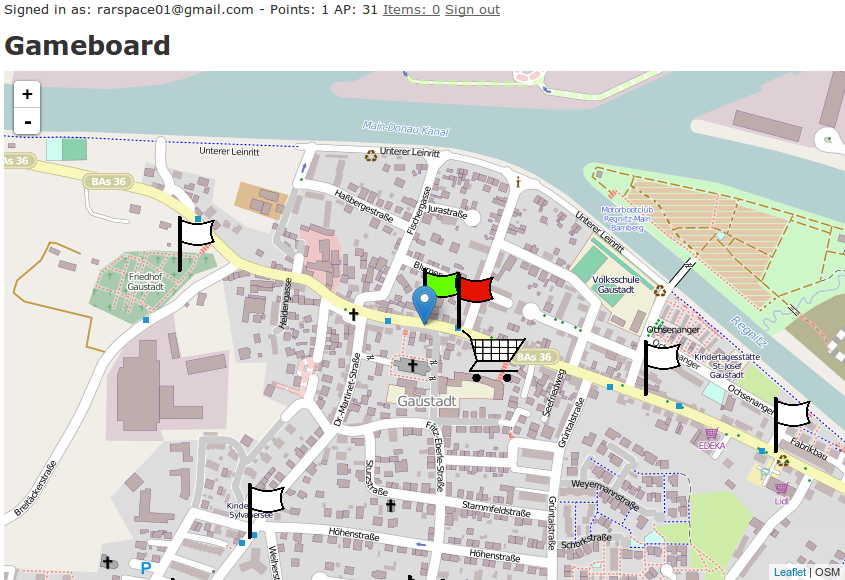
\includegraphics[width=150mm]{images/ch5_img09_gameboard.png}
\caption{Grundansicht - Spielfeld}
\label{img:ch5_img09_gameboard}
\end{center}
\end{figure}

Das Spielfeld ist in Abbildung \ref{img:ch5_img09_gameboard} zu sehen. In der initialen Sicht wird das Spielfeld mittels HTML5 Geo Api auf die aktuelle Position zentriert. Die Karte selbst zeigt die Standard OSM Tiles. Diese können beliebig ersetzt werden. Gerade in Innenstädten kann es Sinn machen, entsprechend ein anderes Rendering zu verwenden. Eine Übersicht der kostenlosen Tileserver ist unter \url{http://wiki.openstreetmap.org/wiki/Tiles} zu finden. Möchte man über diese hinaus andere Styles verwenden und nicht selbst ein entsprechenden Tile-Renderingserver aufsetzten, so ist es zu empfehlen auf entsprechende Dienste wie z.B. MapBox\footnote{\url{https://www.mapbox.com/}} zurückzugreifen. Auf der Karte selbst sind per Layer die entsprechenden Spielelemente, sowie Händler eingebunden. Bewegt der Spieler den Kartenbereich oder bewegt er sich physikalisch fort, so werden die Daten entsprechend nachgeladen. Die Daten werden mittels GameAPI über das Framework ausgelesen und als GeoJSON eingebunden. Möchte nun der Spieler mit den entsprechenden Spielelementen interagieren, so muss er nur auf das entsprechende Element klicken. Im Beispielspiel öffnet sich dann je nach Elementtyp entweder die Übersicht der jeweiligen Flagge oder aber der Händler. Durch die Interaktion kann sich der Spiele über den aktuellen Prestige-Stnd informieren, sowie die Flagge angreifen. Dies kann der Spieler allerdings nur, wenn er sich im Umkreis von 40 Metern zur Flagge befindet. Beim AJAX Request, welcher der Spieler bei einem Angriff entsprechend durchführt, wird dieses sichergestellt. Der Aktionradius von 40 Meter soll sicherstellen, dass auch bei einer höheren GPS-Ungenaugikeit der Spieler trotzdem mit der Umgebung interagieren kann.
Beim Händler erhält der Spieler eine Übersicht über die verfügbaren Items. Im Gegensatz zu den Flaggen werden die Informationen über die jeweiligen Händler nicht direkt bei dem Abruf aller Händler mitgeteilt, sondern explizit für den jeweiligen Händler angefordert. Somit wird sichergestellt, dass die Synchronisierung möglichst zeitnah ist und der Spieler eine aktuelle Übersicht über das Inventars des virtuellen Händlers erhält.

Den aktuellen Punktestand kann der Spieler von der oberen Statusleiste entnehmen. Dieser berechnet sich anhand aller Flaggen die der Spieler eingesammelt hat. Dank Active Record in Verbindung mit Rails kann die Abfrage stark vereinfacht werden werden:
\\
\lstset{
   language=Ruby
}

\begin{lstlisting}[caption=Ruby - Abfrage der Spielerpunkte, label=code:ch5:activerecord01]
points = Flag.sum(:prestige, :conditions => ['user_id = ?',self.id])
\end{lstlisting}

Direkt daneben ist die Anzeige für die verbliebenen Aktionspunkte. Diese werden alle 60min um eins erhöht bis diese 24 Aktionspunkte erreichen. Der letzte Punkt stellt die Item-Übersicht dar. Über diese kann der Spieler seine aktuellen Items sich anzeigen lassen und je nach Bedarf diese auch entsprechend verwenden. Die Items werden erst mit dem klick auf das Inventar explizit per AJAX nachgeladen. zuvor kann der Spieler jedoch die Anzahl seiner Items in der Statusleiste sehen.
\\\\
Im Gegenzug dazu gibt es die Oberfläche für die Pflege der einzelnen Händler. Hierfür werden als Basis, durch Scaffolding generierte Formulare verwendet. Diese wurden entsprechend um zusätzliche Funktionen wie einem Leaflet map picker, sowie der dazugehörige JavaScript Code ergänzt. Zunächst kann der Spielleiter sich eine Übersicht der Händler über die nachfolgende Url aufrufen:
\\\\
\url{SITE\_URL/vendors}
\\\\
In der Übersicht kann er bestehende Händler direkt löschen, Neue anlegen oder Bestehende bearbeiten. 
Legt der Spielleiter einen Händler an, so wird ihm nicht nur eine Liste an Attributen angezeigt, sondern er erhält auch eine Leaflet Karte, die entsprechend auf der aktuellen Position zentriert ist. Über diese kann er frei auf der Karte einen Marker für die Position des Händlers setzen. Intern werden die Koordinaten des Markers entsprechend gespeichert und in der Datenbank hinterlegt. Möchte der Spielleiter nun einen der Händler bearbeitne wird analog dazu das FOrmular wieder aufgerufen und entsprechend mit den Daten aus der Datenbank gefüllt. Gleiches gilt auch für die Leaflet Karte auf der der zuvor gespeicherte Marker hinterlegt wurde. In diesem Mdus hat der Spielleiter zudem die Möglichkeit Items direkt dem Händler zuzuweisen die dann später zum Verkauf stehen. Für die Einfachheit werden entsprchend alle freien noch nich zugewiesenen Items entsprechend angezeigt und können mit einem einfachen Klick hinzugefügt werden. Hierfür sind entsprechende Controller für die Händler Klasse erstellt worden, die das Kaufen und Zuweisen von Items ermöglichen.

Über die nachfolgende Unterseite, findet die Pflege der Items statt:
\\\\
\url{SITE\_URL/items}
\\\\
Auf dieser Seite erstellt der Spielleiter alle Items die den Händlern zur Verfügung stehen sollen. Hierbei handelt es sich ebenfalls um ein nach typischen Scaffolding erzeugtem Formularmuster zur Pflege der einzelnen Daten. Jedes Item ist dabei explizit als Objekt angelegt und kann einem Itemtyp angehören. Eine Anpassung der Items ist nach der Erstellung möglich. Im Zuge des Beispielspiels wurde auf eine umfangreiche Rollen und Rechtevergabe verzichtet, da der Fokus auf den Spielelemente lag. Nichtsdestotrotz können diese entsprechend erweitert werden, je nachdem für welches Spiel das Framework eingesetzt werden soll.

\subsubsection*{Evaluationstool}

Das Evalutationstool verwendet die zuvor in der GameAPI beschriebene Schnittstelle um Spielfelder zu bewerten bzw. zu evaluieren. Hierfür wird die zusätzliche Möglichkeit genutzt konkrete tags zu einer Bounding Box abzufragen. Für eine Evaluation verwendet das Tool eine vorgegebene Liste an Key-Value Paaren und eine Geo-Koordinate, die zu einer Bounding Box erweitert wird. Basierend auf dem im Kapitel \ref{ch:CH6_qualtiy_of_gameboards} beschriebenen Ansätzen werden die einzelnen Spielfelder jeweils Evaluiert. Für die Evaluation der Spielfelder müssen die Entfernung zwischen den einzelnen Punkten berechnet werden. Hierbei werden nicht die euklidische Distanz zwischen den Geo-Koordinaten berechnet sondern es muss die reale Netzwerkdistanz auf dem Straßennetz berechnet werden. Da der Spieler nicht nur per Auto sondern bevorzugt auch per Fahrrad und im besten Fall zu Fuß das Spiel nutzt, ist ein Fußgängerrouting notwendig. Das bedeutet Wege die nur für Fußgänger zugänglich sind, müssen ebenfalls beachtet werden. Da Openstreetmap im Vergleich zu Google Maps im Hinblick auf den Datenumfang an dieser Stelle einen Vorteil hat, ist es sinnvoll hierfür auf OSM zurückzugreifen. Durch den Umfang und Anzahl der Abfragen die sich durch die Evaluationsmethoden ergeben, ist es sinnvoll die Anfragen nicht an einen Onlinedienst zu stellen sondern diese offline mit einem dedizierten Routing durchzuführen. Für das offline Routing mit OSM gibt es diverse Bibliotheken, aufgrund der Anforderung möglichst viele Abfragen zeitnah durchzuführen wurde sich für das Tool GraphHopper entschieden. Dieses bietet ein vollständiges Offline Routing auf Basis von OSM Rohdaten \cite{Karich.2014}. Hierfür erstellt GraphHopper zunächst entsprechende Indexdateien auf denen dann später das Routing stattfindet. Diese enthalten in binärer Form die agregierten Pfade des Netzwerkes.

Mit Hilfe von GraphHopper ist es nun Möglich entsprechend schnelle Abfragen durchzuführen. Da die GraphHopper Bibliothek selbst nicht für Parallelisierung ausgelegt ist, wurde das Evaluationstool entsprechend optimiert um die Ressourcen eines Rechners/Servers vollständig auszunutzen. Dadurch kann die Laufzeit bei mehreren Tags je nach Anzahl der vorhandenen CPUs auf $\frac{1}{lc}$ verkürzt werden. Wobei lc die Anzahl der logischen CPUs darstellt. Bei einer Laufzeit von $\mathcal O(n^2)$ ist dies unerlässlich.
Da GraphHopper in Java realisiert wurde, wurde das Evaluationstool analog dazu ebenfalls in Java entwickelt.

\subsection*{Tests}

Da das Framework später entsprechend für verschiedene Spiele genutzt werden soll, muss dieses entsprechend getestet werden.
Hierbei wird unterschieden zwischen Low-Level-Tests und High-Level-Tests\cite{Pol.2002},
Unter Low-Level-Tests sind solche Test zu verstehen, die während der Implementierung an Teilen des Systems stattfinden. Bei High-Level-Tests wird das komplette System getestet. Einer der Low-Level-Tests ist der Modultest. Bei diesem werden einzelne Module im Programm getestet.  

Für das Gameframework wurden die einzelnen Module unabhängig voneinander getestet. Zunächst wurden speziell die Schnittstellen zu OSM und Overpass getestet. Hierbei wurde vor allem kontrolliert, dass die Übergabeparameter, sowie das Datenformat korrekt ist und die Interpretation der Daten korrekt vorgenommen wird.
Nachdem die die GameAPI mit ihrer Transformation der OSM Elemenete in Spielelemente implementiert wurde, ist das Beispielspiel entsprechend darauf aufgebaut worden. Hierzu wurde die korrekte Transformation der Elemente anhand von speziellen Tags manuell überprüft. Hierzu wurde \url{http://taginfo.openstreetmap.org} verwendet. Dies Seite bietet einen statistischen Überblick aller tags in OSM sowie die Verteilung auf die Elemente Relation, Way und Nodes. Der Test erfolge anhand von Key-Value Paaren die jeweils explizit nur als einer der drei Typen bevorzugt gemappt werden.

Das Spiel selbst musste ebenfalls getestet werden. Da ein ortsbezogenes Spiel als Grundlage die Position de Spielers verwendet und ein Debugging unterwegs sich als schwierig gestaltet, ist es am besten die GPS-Koordinate zu simulieren. Hierfür gibt es entsprechende Plugins für die am weitesten verbreiteten Browser, wie Chrome oder Firefox. mit Hilfe von diesen kann die Position welche die HTML5  Geo API zurückliefert entsprechend verändert werden. Darüber hinaus ist es auch möglich die Genauigkeit der GPS Position, sowie das Bewegungs-Event zu triggern. Mit Hilfe von diesem können alle ortbezogenen Funktionen des Beispielspiels auch dirke twährend der Entwicklung getestet werden.
Für die Nutzung des Spieles auf Smartphones eignet sich darüberhinaus der Einsatz von entsprechenden Emulatoren. Für Android und FirefoxOS sind diese frei verfügbar. Für iOS fallen jährliche Gebühren an und der Emulator inkl. SDK ist nur unter der neusten Mac OS X Version verfügbar.

Tests für das Evaluationstool wurden vorwiegend für die Performance und den Werten durchgeführt.
Konkrete Unit-Tests wurden für das Framework aus Zeitgründen nicht entwickelt, sollten aber als nächster wichtiger Punkt entsprechend implementiert werden.

Als High-Level bzw. Blackbox Test wurden die in den Usecase Diagramm beschriebenen Anwendungsfälle getestet. D.h. die Funktionen die den jeweiligen Akteuren zur Verfügung stehen wurden ohne Betrachtung.

\subsection*{Probleme}

Während der Umsetzung sind auf einige Besonderheiten gestoßen, welche eine spezielle Anpassung oder Überlegung erfordert haben. Im nachfolgenden soll kurz auf diese eingegangen werden um die Erkenntnisse festzuhalten. Idealerweise können diese in zukünftigen Untersuchungen und Implementierungen entsprechend vermieden bzw. umgangen werden.

Ein erster Aspekt der von Relevanz, ist die Spezifikation der GeoJSON. Standardmäßig werden Koordinaten in der Reihenfolge Latitude, Longitude angegeben \cite{Schoeneberger.2002,Barzegar.1996,Maling.1991,}. Die GeoJSON Spezifikation hingegen sieht im Kontrast zum de facto Standard vor, dass zuerst die Longitude und dann die Latitude genannt wird \cite{Butler.2008}. Ist dies nicht bekannt, kann dies zu einigem Aufwand führen, der vermeiden werden kann.

Ein weiteres Problematik die im Zuge des Transformationsprozesses der Relations und Ways zu virtuellen Nodes mit einer mit Bitmasken codierten Eigenschaft, führte dazu, dass im Zuge der Verwendung mit Javascript Probleme auftraten. Dies äußerte sich darin, dass die Ids nach der Interpreation plötzlich auf unerklärlicher weise veränderte Werte annahmen. So kamen Abweichungen von bis zu 100 zu Stande. Nach längeren Debug Aufwänden wurde herausgefunden, dass die implizite Typisierung in JavaScript den Ganzzahlenwert der Id intern als Gleitkommazahl transferiert und dadurch unbewussterweise die 51Bit überschreitet nach denen die Mantisse der Gleitkommazahl beginnt. Durch diese Verschiebung wurden die hinteren Bits beim auslesen des long Wertes vernachlässigt. Um dieses Problem zu umgehen gibt es zwei Möglichkeiten. Entweder man teilt die Zahl auf Basis des 64bit long Wertes in zwei 32bit Integer Werte und legt diese in zwei Zahlen in JS ab. Sollten keine arithmetischen Operationen auf der Id durchgeführt werden sollen im JavaScript Code, dann empfiehlt es sich die Id explizit als String auszugeben, damit JavaScript diese nicht als Zahl interpretiert und versucht entsprechend umzuwandeln.

Ein weiterer Punkt stellt Turbolinks dar. Turbolinks ist ein Gem, welches Standardmäßig in Rails aktiv ist. Es sorgt dafür, dass bei einer Interaktion mit der Seite nicht die komplette Seite neu geladen wird, sondern nur die Teile des Html Codes, welcher sich geändert hat \cite{Gamble.2013}. Die Problematik die damit einhergeht sind Ajax Requests, welche über normale href links angestoßen werden. Eine typische Verwendung ist z.B.:
\lstset{
   language=Html
}

\begin{lstlisting}[caption=a href HTML Code, label=code:ch5:html01]
<a href='#' onClick="saveItem(1);">Save</a>
\end{lstlisting}

Allerdings für der Klick auf "Save" in diesem Fall zu einem Neuladen der Seite durch Turbolinks. Befindet sich an dieser Stelle aber ein Javascriptcode mit Ajax request, passiert es, dass die Seite neu geladen wird anstatt den Code auszuführen, welcher z.B. eine Aktualisierung einer Zahl auf der Seite zur Folge hätte.
Um diese zu vermeiden muss Turbolinks explizit angewiesen werden, bei a href Links nicht aktiv zu werden. Dies kann man pro Link individuell setzten:

\begin{lstlisting}[caption=a href HTML Code - Turbolinks deaktiviert, label=code:ch5:html01]
<a href='#' data-no-turbolink onClick="saveItem(1);">Save</a>
\end{lstlisting}

Dadurch wird sichergestellt, dass der entsprechende JavaScript Code ausgeführt wird und nicht einfach die Seite neugeladen wird.

Ein letzter Punkt, der zu Problemen führen kann ist der "Zurück"-Button im Browser.
Durch diesen wird die vorherige Seite wieder aufgerufen, allerdings deren Javascriptcode nicht nocheinmal 1:1 getriggert wie beim laden der Seite. D.h. diverse Eventlistener welche auf "OnDocumentReady" z.B. mittels JQuery warten, werden nicht noch einmal aufgerufen. Wird dies nicht entsprechend in der Entwicklung berücksichtigt, kann es dazu führen, dass die Seite sich in einem nicht definierten Zustand befindet.